\documentclass{article}

\usepackage{beamz}
\usepackage{siunitx}
\usepackage{verbatim}
\usepackage{float}
\usepackage{hyperref}



\title{beamz.sty}
\author{Filip Nilenius}


\begin{document}
\maketitle
\begin{abstract}
\texttt{beamz.sty} lets you draw beams with arbitrary loading and support conditions directly in your \LaTeX{} document in a parameterized fashion. Shear force and bending moment diagrams are also supported. \texttt{beamz.sty} uses PGF/Ti\textit{k}z to produce graphics and is ultimately only a set of \texttt{\textbackslash newcommand}s.
\end{abstract}

\tableofcontents

\section{Beam}
The basic command is \texttt{\textbackslash beam\{<length>\}\{<height>\}} which needs to be encapsulated within a \texttt{tikzpicture} environment.

\paragraph{Example}:
\begin{figure}[H]
\centering
\begin{tikzpicture}
\beam{5}{0.2}
\end{tikzpicture}
\end{figure}
\begin{verbatim}
\begin{tikzpicture}
\beam{5}{0.2}
\end{tikzpicture}
\end{verbatim}

All other objects (eg supports and loads) need the beam as a reference so the command \texttt{\textbackslash beam} should be provided before anything else is drawn.

\section{Supports}
The following supports are implemented:
\begin{itemize}
\item Triangle supports: \texttt{\textbackslash triangleSupport{<rel.pos.>}}
\item Roller supports: \texttt{\textbackslash rollerSupport{<rel.pos.>}}
\item Clamped supports:
\begin{itemize}
\item \texttt{\textbackslash clampedLeft{<height>}{<thickness>}}
\item \texttt{\textbackslash clampedRight{<height>}{<thickness>}}
\end{itemize}
\end{itemize}

The height of \texttt{\textbackslash triangleSupport} and \texttt{\textbackslash rollerSupport} are set by the command \texttt{\textbackslash setSupportHeight\{<height\}} which needs to be given before  any support is drawn.

\paragraph{Example}:
\begin{figure}[H]
\centering
\begin{tikzpicture}
% beam
\beam{5}{0.2}

% supports
\setSupportHeight{0.4}
\triangleSupport{0.2}
\rollerSupport{0.5}
\rollerSupport{0.8}
\clampedLeft{0.4}{0.1}
\clampedRight{0.4}{0.1}
\end{tikzpicture}
\end{figure}
\begin{verbatim}
\begin{tikzpicture}
% beam
\beam{5}{0.2}

% supports
\setSupportHeight{0.4}
\triangleSupport{0.2}
\rollerSupport{0.5}
\rollerSupport{0.8}
\clampedLeft{0.4}{0.1}
\clampedRight{0.4}{0.1}
\end{tikzpicture}
\end{verbatim}

\section{Joint}
A joint can be added to the beam using the command \texttt{\textbackslash joint\{<rel. pos.>\}}. The joint's size is proportional to the beam's thickness.

\paragraph{Example}:
\begin{figure}[H]
\centering
\begin{tikzpicture}
%beam
\beam{5}{0.2}

% joint
\joint{0.5}

%supports
\setSupportHeight{0.4}
\clampedLeft{0.4}{0.1}
\rollerSupport{1.0}
\end{tikzpicture}
\end{figure}
\begin{verbatim}
\begin{tikzpicture}
%beam
\beam{5}{0.2}

% joint
\joint{0.5}

%supports
\setSupportHeight{0.4}
\clampedLeft{0.4}{0.1}
\rollerSupport{1.0}
\end{tikzpicture}
\end{verbatim}

\section{Loads}
\subsection{Point loads}
The command \texttt{\textbackslash pointLoad} takes 5 arguments:\\
\texttt{\textbackslash pointLoad\{<rel.pos.>\}\{<height>\}\{<annotation>\}\{<annotations pos.>\}\{<vertical offset>\}}

\paragraph{Example}:
\begin{figure}[H]
\centering
\begin{tikzpicture}
% beam
\beam{5}{0.2}

% loads
\pointLoad{0.2}{1.0}{$P_1$}{left}{0}
\pointLoad{0.8}{1.0}{$P_2$}{right}{0}
\pointLoad{0.6}{1.0}{$P_3$}{above}{0}

% supports
\setSupportHeight{0.4}
\triangleSupport{0.0}
\rollerSupport{0.7}
\rollerSupport{1.0}
\end{tikzpicture}
\end{figure}
\begin{verbatim}
\begin{tikzpicture}
% beam
\beam{5}{0.2}

% loads
\pointLoad{0.2}{1.0}{$P_1$}{left}{0}
\pointLoad{0.8}{1.0}{$P_2$}{right}{0}
\pointLoad{0.6}{1.0}{$P_3$}{above}{0}

% supports
\setSupportHeight{0.4}
\triangleSupport{0.0}
\rollerSupport{0.7}
\rollerSupport{1.0}
\end{tikzpicture}
\end{verbatim}

\subsection{Point moment}
The commands \texttt{\textbackslash momentClockwise} and \texttt{\textbackslash momentCounterclockwise} both take the same 6 arguments:\\
\texttt{\textbackslash momentClockwise\{<rel.pos.>\}\{<radius>\}\{<start angle>\}\{<delta angle>\}\{<annotation>\}\\\{<annotation pos.>\}}
\paragraph{Example}:
\begin{figure}[H]
\centering
\begin{tikzpicture}
% beam
\beam{5}{0.2}

% loads
\momentClockwise{1.0}{0.5}{-30}{100}{$M_1$}{right}
\momentCounterclockwise{0.0}{0.5}{120}{90}{$M_3$}{left}
\momentCounterclockwise{0.5}{0.5}{45}{90}{$M_2$}{above}

% supports
\setSupportHeight{0.4}
\triangleSupport{0.0}
\rollerSupport{0.7}
\rollerSupport{1.0}
\end{tikzpicture}
\end{figure}

\begin{verbatim}
\begin{tikzpicture}
% beam
\beam{5}{0.2}

% loads
\momentClockwise{1.0}{0.5}{-30}{100}{$M_1$}{right}
\momentCounterclockwise{0.0}{0.5}{120}{90}{$M_3$}{left}
\momentCounterclockwise{0.5}{0.5}{45}{90}{$M_2$}{above}

% supports
\setSupportHeight{0.4}
\triangleSupport{0.0}
\rollerSupport{0.7}
\rollerSupport{1.0}
\end{tikzpicture}
\end{verbatim}

\subsection{Distributed loads}
\subsubsection{Rectangle loads}
The command \texttt{\textbackslash distributedload} takes 6 arguments:\\
\texttt{\textbackslash distributedload\{<start pos.>\}\{<end pos.>\}\{<annotation left>\}\{<annotation right>\}\{<height>\}\{<vertical offset>\}}

\paragraph{Example}:
\begin{figure}[H]
\centering

\begin{tikzpicture}
% beam
\beam{5}{0.2}

% loads
\distributedLoad{0.0}{1.0}{$W_1$}{}{0.8}{0}
\distributedLoad{0.5}{1.0}{$W_2$}{}{0.8}{1}

% supports
\setSupportHeight{0.4}
\triangleSupport{0.0}
\rollerSupport{0.5}
\rollerSupport{1.0}
\end{tikzpicture}
\end{figure}
\begin{verbatim}

\begin{tikzpicture}
% beam
\beam{5}{0.2}

% loads
\distributedLoad{0.0}{1.0}{$W_1$}{}{0.8}{0}
\distributedLoad{0.5}{1.0}{$W_2$}{}{0.8}{1}

% supports
\setSupportHeight{0.4}
\triangleSupport{0.0}
\rollerSupport{0.5}
\rollerSupport{1.0}
\end{tikzpicture}
\end{verbatim}

\subsubsection{Triangle loads}
The commands \texttt{\textbackslash triangleloadLeft} and \texttt{\textbackslash triangleloadRight} both take the same 6 arguments:\\
\texttt{\textbackslash triangleloadLeft\{<start pos.>\}\{<end pos.>\}\{<annotation>\}\{annotation pos.>\}\{<height>\}\{<vertical offset>\}}

\paragraph{Example}:
\begin{figure}[H]
\centering
\begin{tikzpicture}
% beam
\beam{5}{0.2}

% loads
\distributedLoad{0.6}{1.0}{}{$W_1$}{0.4}{0}
\triangleloadLeft{0.0}{0.4}{$W_2$}{above}{1.0}{0}
\triangleloadRight{0.6}{1.0}{$W_3$}{right}{1.0}{0.55}

% supports
\setSupportHeight{0.4}
\triangleSupport{0.0}
\rollerSupport{0.7}
\rollerSupport{1.0}
\end{tikzpicture}
\end{figure}
\begin{verbatim}
\begin{tikzpicture}
% beam
\beam{5}{0.2}

% loads
\distributedLoad{0.6}{1.0}{}{$W_1$}{0.4}{0}
\triangleloadLeft{0.0}{0.4}{$W_2$}{above}{1.0}{0}
\triangleloadRight{0.6}{1.0}{$W_3$}{right}{1.0}{0.55}

% supports
\setSupportHeight{0.4}
\triangleSupport{0.0}
\rollerSupport{0.7}
\rollerSupport{1.0}
\end{tikzpicture}
\end{verbatim}

\section{Annotation}
\subsection{Dimension annotations}
\texttt{\textbackslash dimension\{<start pos.>\}\{<end pos.>\}\{<vertical disp.>\}\{<annotation>\}\{<dashed line extension>\}}\\
where \texttt{<dashed line extension>} is a fraction of \texttt{<vertical disp.>}.

\paragraph{Example}:
\begin{figure}[H]
\centering
\begin{tikzpicture}
% beam
\beam{5}{0.2}

% loads
\pointLoad{0.4}{1.0}{$P$}{left}{0}

% supports
\setSupportHeight{0.4}
\triangleSupport{0.0}
\rollerSupport{1.0}

% dimensions
\dimension{0.0}{0.4}{1.0}{$aL$}{0.5}
\dimension{0.4}{1.0}{1.0}{$(1-a)L$}{0.5}
\dimension{0.0}{1.0}{1.7}{$L$}{0.0}
\end{tikzpicture}
\end{figure}
\begin{verbatim}
\begin{tikzpicture}
% beam
\beam{5}{0.2}

% loads
\pointLoad{0.4}{1.0}{$P$}{left}{0}

% supports
\setSupportHeight{0.4}
\triangleSupport{0.0}
\rollerSupport{1.0}

% dimensions
\dimension{0.0}{0.4}{1.0}{$aL$}{0.5}
\dimension{0.4}{1.0}{1.0}{$(1-a)L$}{0.5}
\dimension{0.0}{1.0}{1.7}{$L$}{0.0}
\end{tikzpicture}
\end{verbatim}

\subsection{Beam annotation}
Beam annotations can be added using the commands:\\
\begin{itemize}
\item \texttt{\textbackslash beamAnnotationBelow\{<rel.pos.>\}\{<annotation>\}} 
\item \texttt{\textbackslash beamAnnotationAbove\{<rel.pos.>\}\{<annotation>\}}
\end{itemize}

\paragraph{Example}:
\begin{figure}[H]
\centering
\begin{tikzpicture}
% beam
\beam{5}{0.2}

% loads
\pointLoad{0.4}{1.0}{$P$}{left}{0}

% supports
\setSupportHeight{0.4}
\triangleSupport{0.0}
\rollerSupport{1.0}

% annotation
\beamAnnotationAbove{0}{A}
\beamAnnotationAbove{1}{B}
\beamAnnotationBelow{0.5}{$EI$}
\end{tikzpicture}
\end{figure}
\begin{verbatim}
\begin{tikzpicture}
% beam
\beam{5}{0.2}

% loads
\pointLoad{0.4}{1.0}{$P$}{left}{0}

% supports
\setSupportHeight{0.4}
\triangleSupport{0.0}
\rollerSupport{1.0}

% annotation
\beamAnnotationAbove{0}{A}
\beamAnnotationAbove{1}{B}
\beamAnnotationBelow{0.5}{$EI$}
\end{tikzpicture}
\end{verbatim}

\section{Coordinate axes}
Coordinate axes for a beam can be drawn using the two commands: 
\begin{itemize}
\item \texttt{\textbackslash horizontalAxis} (draws $x$ axis)
\item \texttt{\textbackslash verticalAxis} (draws $z$ axis (positive direction upwards))
\end{itemize}
The coordinate axes' lengths are proportional to the beam's length and height, respectively.

\paragraph{Example}:
\begin{figure}[H]
\centering
\begin{tikzpicture}
% beam
\beam{5}{0.2}

% loads
\pointLoad{0.4}{1.0}{$P$}{left}{0}

% supports
\setSupportHeight{0.4}
\triangleSupport{0.0}
\rollerSupport{1.0}

% axes
\horizontalAxis
\verticalAxis
\end{tikzpicture}
\end{figure}
\begin{verbatim}
\begin{tikzpicture}
% beam
\beam{5}{0.2}

% loads
\pointLoad{0.4}{1.0}{$P$}{left}{0}

% supports
\setSupportHeight{0.4}
\triangleSupport{0.0}
\rollerSupport{1.0}

% axes
\horizontalAxis
\verticalAxis
\end{tikzpicture}
\end{verbatim}


\section{Reaction forces}
Reaction forces can be drawn using the command \texttt{\textbackslash reactionForce} which takes 3 arguments:

\texttt{\textbackslash reactionForce\{<position>\}\{<annotation>\}\{<annotation pos.>\}}
The arrow's offset distance from the support is proportional to the support's height so the supports need to be drawn before the reaction forces. The hight of the reaction force is set by the command\\
\texttt{\textbackslash setReactionForceHeight\{<height>\}}

\paragraph{Example}:
\begin{figure}[H]
\centering
\begin{tikzpicture}
% beam
\beam{5}{0.2}

% loads
\pointLoad{0.5}{1.0}{$P$}{left}{0}

% supports
\setSupportHeight{0.4}
\triangleSupport{0.0}
\rollerSupport{1.0}

% reaction forces
\setReactionForceheight{0.8}
\reactionForce{0.0}{$\displaystyle\frac{P}{2}$}{right}
\reactionForce{1.0}{$\displaystyle\frac{P}{2}$}{left}
\end{tikzpicture}
\end{figure}
\begin{verbatim}
\begin{tikzpicture}
% beam
\beam{5}{0.2}

% loads
\pointLoad{0.5}{1.0}{$P$}{left}{0}

% supports
\setSupportHeight{0.4}
\triangleSupport{0.0}
\rollerSupport{1.0}

% reaction forces
\setReactionForceheight{0.8}
\reactionForce{0.0}{$\displaystyle\frac{P}{2}$}{right}
\reactionForce{1.0}{$\displaystyle\frac{P}{2}$}{left}
\end{tikzpicture}
\end{verbatim}


\section{Cross-sectional force diagrams}
The commands \texttt{\textbackslash Tofx} and \texttt{\textbackslash Mofx} both take the same 3 arguments:\\
\texttt{\textbackslash Tofx\{<T(x)>\}\{<vertical shift>\}\{<scale factor>\}} where \texttt{\{<T(x)>\}} is $T(x)$ (or $M(x)$) given as a path of either coordinates or analytical functions, or a combination of both (see example below). When analytical expressions are given in \texttt{\{<T(x)>\}}, the true length of the beam needs to be declared for correct scaling of the graph, which is done using the command \texttt{\textbackslash setTrueBeamLength\{<beam length\}}. 

\paragraph{Example}
In the example below $L_1 = \SI{6}{\meter}$ and $L_2 = \SI{2}{\meter}$. The example needs \texttt{\textbackslash usepackage\{siunitx\}} in the preamble.
\begin{figure}[H]
\centering
\begin{tikzpicture}

% Beam
\beam{7}{0.2}

% Force
\triangleloadRight{0}{0.6}{$W_1 = \SI{60}{\kilo\newton\per\meter}$}{right}{1.2}{0}
\distributedLoad{6/10}{1}{}{$W_2 = \SI{40}{\kilo\newton\per\meter}$}{0.8}{0}

% Supports
\setSupportHeight{0.4}
\triangleSupport{0}
\rollerSupport{8/10}

% Dimension
\dimension{0}{6/10}{2}{$L_1$}{0.3}
\dimension{6/10}{8/10}{2}{$L_2$}{0.3}
\dimension{8/10}{1.0}{2}{$L_2$}{0.3}
\dimension{0}{4.24/10}{2.9}{$\SI{4.24}{\meter}$}{0}
\horizontalAxis
\verticalAxis


% Support reactions
\setReactionForceheight{0.8}
\reactionForce{0}{$\SI{90}{\kilo\newton}$}{right}
\reactionForce{8/10}{$\SI{250}{\kilo\newton}$}{left}


\setTrueBeamLength{10}
% T(x)
\Tofx{
(0,-90) node[left] {$\SI{-90}{\kilo\newton}$}
--
plot[domain=0:6] (\x, {5*\x^2-90})
--
(6,90) node[left] {$\SI{90}{\kilo\newton}$}
--
plot[domain=6:8] (\x, {40*(\x-6)+90})
--
(8,170) node[right] {$\SI{170}{\kilo\newton}$}
--
(8,-80) node[left] {$\SI{-80}{\kilo\newton}$}
--
plot[domain=8:10] (\x, {40*(\x-6)-160})
}{4.5}{0.01}

% M(x)
\Mofx{
(0,0)
--
plot[domain=0:4.24] (\x, {-90*\x+5/3*\x^3})
--
(4.24,-255) node[below] {$\SI{-255}{\kilo\newton\meter}$}
--
plot[domain=4.24:6] (\x, {-90*\x+5/3*\x^3})
--
plot[domain=6:8] (\x, {20*(\x-6)^2+90*\x-720})
--
(8,80) node[above] {$\SI{80}{\kilo\newton\meter}$}
--
plot[domain=8:10] (\x, {20*(\x-6)^2-160*\x+1280})
}{7.5}{0.01}

% dimenstions
\setVerticalLineOffset{2.2}
\verticalLine{0}{8}{dashed}
\verticalLine{4.25/10}{8}{dotted}
\verticalLine{6/10}{8}{dotted}
\verticalLine{8/10}{8}{dotted}
\verticalLine{1}{8}{dashed}
\end{tikzpicture}
\end{figure}
\begin{verbatim}
\begin{tikzpicture}

% Beam
\beam{7}{0.2}

% Force
\triangleloadRight{0}{0.6}{$W_1 = \SI{60}{\kilo\newton\per\meter}$}{right}{1.2}{0}
\distributedLoad{6/10}{1}{}{$W_2 = \SI{40}{\kilo\newton\per\meter}$}{0.8}{0}

% Supports
\setSupportHeight{0.4}
\triangleSupport{0}
\rollerSupport{8/10}

% Dimension
\dimension{0}{6/10}{2}{$L_1$}{0.3}
\dimension{6/10}{8/10}{2}{$L_2$}{0.3}
\dimension{8/10}{1.0}{2}{$L_2$}{0.3}
\dimension{0}{4.24/10}{2.9}{$\SI{4.24}{\meter}$}{0}
\horizontalAxis
\verticalAxis


% Support reactions
\setReactionForceheight{0.8}
\reactionForce{0}{$\SI{90}{\kilo\newton}$}{right}
\reactionForce{8/10}{$\SI{250}{\kilo\newton}$}{left}


\setTrueBeamLength{10}
% T(x)
\Tofx{
(0,-90) node[left] {$\SI{-90}{\kilo\newton}$}
--
plot[domain=0:6] (\x, {5*\x^2-90})
--
(6,90) node[left] {$\SI{90}{\kilo\newton}$}
--
plot[domain=6:8] (\x, {40*(\x-6)+90})
--
(8,170) node[right] {$\SI{170}{\kilo\newton}$}
--
(8,-80) node[left] {$\SI{-80}{\kilo\newton}$}
--
plot[domain=8:10] (\x, {40*(\x-6)-160})
}{4.5}{0.01}

% M(x)
\Mofx{
(0,0)
--
plot[domain=0:4.24] (\x, {-90*\x+5/3*\x^3})
--
(4.24,-255) node[below] {$\SI{-255}{\kilo\newton\meter}$}
--
plot[domain=4.24:6] (\x, {-90*\x+5/3*\x^3})
--
plot[domain=6:8] (\x, {20*(\x-6)^2+90*\x-720})
--
(8,80) node[above] {$\SI{80}{\kilo\newton\meter}$}
--
plot[domain=8:10] (\x, {20*(\x-6)^2-160*\x+1280})
}{7.5}{0.01}

% dimenstions
\setVerticalLineOffset{2.2}
\verticalLine{0}{8}{dashed}
\verticalLine{4.25/10}{8}{dotted}
\verticalLine{6/10}{8}{dotted}
\verticalLine{8/10}{8}{dotted}
\verticalLine{1}{8}{dashed}
\end{tikzpicture}
\end{verbatim}











\end{document}